%! Author = wxw85
%! Date = 01/08/2022

\section{Solution}\label{sec:solution}
%**************************************************************

We tried to tackle the problem by designing a deep neural network which is composed by a feature extractor, the transformer and a MLP to predict the pose.
We feed the feature extractor with a sequence of images, we tried both grey-scale and RGB images, in this way, we obtain a sequence of embeddings (both size 512 and 2048), the embedding are then fed into the transformer (both encoder-only and encoder-decoder version) and the output of the transformer is fed into the MLP to predict the sequence of poses.

\begin{figure}[H]
    \centering
    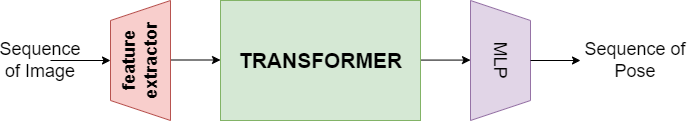
\includegraphics[width=0.8\textwidth]{images/1_4_general_solution}
    \caption{General representation of the model.}
    \label{fig:figure-1_4_solution}
\end{figure}

We use a sequence of image because the transformer model, originally designed for the machine translation, it requires as input a sequence of embeddings, then it outputs another sequence of embeddings.
For major details about the transformer, we refer to \hyperref[sec:exp-models]{\S4.1 Experiments - Models} and \hyperref[sec:models]{\S5.3 Implementation - Models}.